\documentclass[12pt,letterpaper,noanswers]{exam}
\usepackage[usenames,dvipsnames,svgnames,table]{xcolor}
\usepackage[margin=0.9in]{geometry}
\renewcommand{\familydefault}{\sfdefault}
\usepackage{multicol}
\usepackage{wrapfig}
\pagestyle{head}
\definecolor{c03}{HTML}{FFDDDD}
\header{AM 22b Class 18}{}{Mar 12: Parameterization p.\thepage}
\runningheadrule
\pagenumbering{arabic}
\headrule
\usepackage{graphicx} % more modern
\usepackage{amsmath} 
\usepackage{amssymb} 
\usepackage{hyperref}
\usepackage{tcolorbox}

\usepackage[numbered,autolinebreaks,useliterate]{mcode}

\newcommand{\mb}[1]{\underline{#1}}

\begin{document}
 \pdfpageheight 11in 
  \pdfpagewidth 8.5in




% I need to review the torus trajectories...

\begin{itemize}
% \item There is a pre-class assignment (20 minutes of videos + a few WeBWorK exercises) due at 10am this Monday.  It is available on Canvas.
\itemsep0em
    % \item PSet 02 is due on Friday Feb 14th at 10am.
   % \item There is a pre-class assignment due Monday by 10am (pre-class 03).
    \item The next skill check will be for C16, C17, C18 on Monday Mar 15th.
    \item There will be a pre-class assignment for Monday Mar 15th.
    \item Quiz 03 will be posted on Friday Mar 19th.
    \item There will be a short discussion board post due on Thursday Mar 18th, but there is not a problem set this week.
   % \item On the back of the skill check on Friday will be a skill check retake for the C05 skill check.  I will provide an additional retake for C10 at a later date.  (These are skills where $\geq 20\%$ of the class has not satisfied the skill).
\end{itemize}

\hrule
\vspace{0.2cm}

% partial derivatives, gradient
% local linearity, differential, directional deriv
% 2nd order partials + equations with partials

\noindent\textbf{Big picture}

Today is focused on parameterized curves, and on velocity along curves.  Then we'll look at vector fields before returning to integration (with these new functions).

\vspace{0.2cm}
\hrule
\vspace{0.2cm}



\noindent\textbf{Skill Check Practice}
\begin{questions}
\question (velocity) Find $\mb v(t)$ for $\mb{r}(t) = t\mb i + t^2\mb j + t^3\mb k$.
\end{questions}


\vspace{0.2cm}
\hrule
\vspace{0.2cm}

\noindent\textbf{Skill Check Practice Solution}
\begin{questions}
\question $\mb v(t) = \frac{d\mb r}{dt} = \langle 1,2t,3t^2\rangle$.
\end{questions}


\vspace{0.2cm}
\hrule
\vspace{0.2cm}

\noindent\textbf{Teams}

You will work with this team on the in-class problems today.

\begin{multicols}{2}
1.  students here

\end{multicols}


%\vspace{0.2cm}
\hrule
\vspace{0.2cm}



\noindent\textbf{Parameterizing line segments} \S 17.1 
\begin{tcolorbox}
\begin{itemize}
\itemsep0em
    \item \textbf{Line segments} can be parameterized by the three equations \[x = x_0 + a t, \quad y = y_0 + b t, \quad z = z_0 + c t, \quad t_0 \leq t \leq t_1. \]
    \item The vector $\mb v = a\mb i +b\mb j + c\mb k$ is parallel to the line parameterized by $\mb r(t) = (x_0+at)\mb i + (y_0 + bt)\mb j + (z_0 + ct)\mb k = \mb r_0 + t\mb v$ where $\mb r(0) = x_0\mb i + y_0\mb j + z_0\mb k$ is interpreted as a position.
    \item A section of the curve given by the graph of $y = f(x)$ in $\mathbb{R}^2$ can be parameterized by $x = t,$ $y = f(t)$, $a\leq t\leq b$, or $\mb r(t) = t\mb i + f(t)\mb j$, $a\leq t\leq b$.
\end{itemize}
\end{tcolorbox}



\noindent\textbf{Point at time zero}.  What point does the line $\mb r(t)=(3+t)\mb i + 2t\mb j+ (-4-t)\mb k$ pass through when $t=0$?

%\emph{pollQ}

\vspace{1cm}

\noindent\textbf{Vector parallel to line}.
Find a vector aligned parallel to the line $\mb r(t)=(3+t)\mb i + 2t\mb j+ (-4-t)\mb k$.

\vspace{1cm}



\noindent\textbf{Piece of graph of function}

The curve below is a parabola with minimum at $(0,0)$.

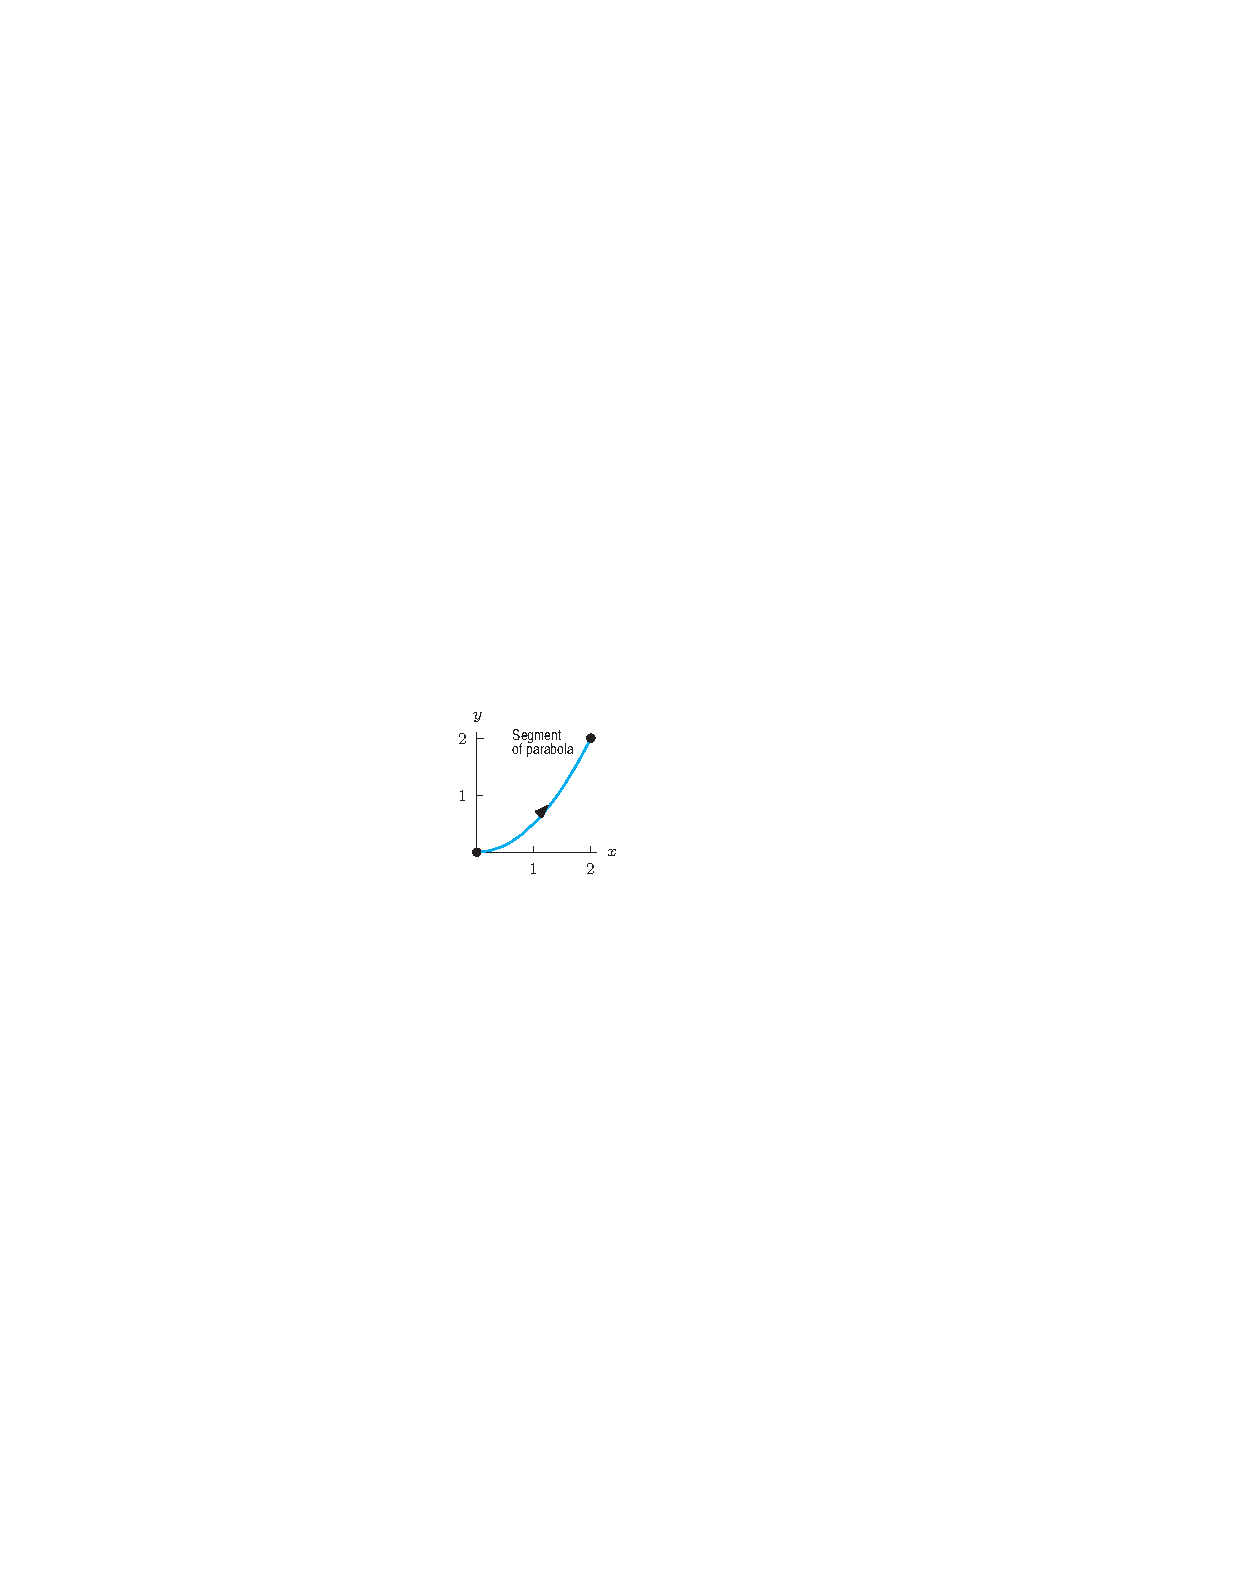
\includegraphics{img/N22_c4.pdf} 

Find a function such that the curve above is a piece of the function $y = f(x)$ and then create a parameterization of the curve. 

\vspace{2in}

\vspace{0.2cm}
\hrule
\vspace{0.2cm}

\textbf{Velocity, speed, tangents}.  \S 17.2 
\begin{tcolorbox}
\begin{itemize}
\itemsep0em
    \item For a particle moving along a parameterized curve with position $(x(t),y(t),z(t))$ (also written $\mb r(t)$),
the \textbf{velocity vector}, $\mb v$, is given by \[\mb v(t) = \frac{dx}{dt} \mb i + \frac{dy}{dt}\mb j + \frac{dz}{dt}\mb k, \text{ also written }\frac{d\mb r}{dt}\text{ or }\mb r'(t).\] 
\item The velocity vector is always interpreted as assigning a vector in $3$-space to each point in time.  It is usually drawn with its tail at $(x(t), y(t), z(t))$. 
\item The \textbf{speed} of a particle along the path $(x(t), y(t), z(t))$ is given by $\Vert \mb v \Vert$.
\item The direction of the velocity vector is the instantaneous direction of motion of the particle. 
\item The velocity vector $\vec v(t)$ drawn with its tail at $\mb r(t)$ is tangent to the path of the object at that point.
\end{itemize}
\end{tcolorbox}
\begin{tcolorbox}
\begin{itemize}
\itemsep0em

\item A unit vector that is tangent to the curve (a \textbf{unit tangent vector}) at the point $\mb r(t)$ is given by
\[\mb T = \frac{\mb v(t)}{\Vert \mb v(t) \Vert} = \left(\frac{1}{\left\Vert d\mb r(t)/dt\right\Vert}\right)\frac{d\mb r}{dt}(t).\] 

\item The acceleration vector $\mb a$ is given by
\[\mb a(t) = \frac{d^2x}{dt^2}\mb i + \frac{d^2y}{dt^2}\mb j + \frac{d^2z}{dt^2}\mb k.\]
\end{itemize}
\end{tcolorbox}

\noindent\textbf{Example (velocity on an ellipse)}.   Let $x(t) =  \cos t$, $y(t) = 2\sin t$ and $z(t) = t$.  Find the velocity vector $\mb v(t)$, the speed $\Vert \mb v(t) \Vert$, and the acceleration vector $\mb a(t)$. 

\begin{multicols}{2}
\begin{lstlisting}
syms t
fplot3(cos(t),2*sin(t),t,[0,2*pi])
xlabel('x'); ylabel('y'); zlabel('z');
hold on
for t0 = pi/2:pi/2:3*pi/2
    x0=cos(t0); y0=2*sin(t0); z0 = t0;
    v1 = [-sin(t0), 2*cos(t0), 1];
    a1 = [-cos(t0), -2*sin(t0), 0];
    plot3([x0,x0+v1(1)],[y0,y0+v1(2)],...
        [z0,z0+v1(3)],'k')
    plot3([x0,x0+a1(1)],[y0,y0+a1(2)],...
        [z0,z0+a1(3)],'r')
end
\end{lstlisting}

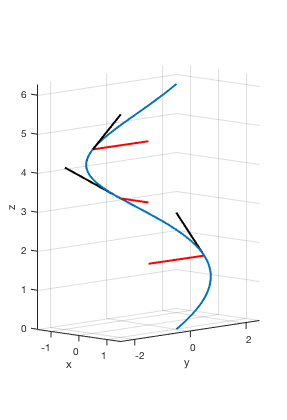
\includegraphics[width=2in]{img/C23p3-18.png}


\end{multicols}

\vfill
%\eject


\noindent\textbf{Motion on a line}.  Let $\mb r(t) = (x_0+at)\mb i + (y_0 + bt)\mb j + (z_0+ct)\mb k$.  This curve is a line.  Find $\mb v(t)$.


\vspace{1in}

\vspace{0.2cm}
\hrule
\vspace{0.2cm}
\noindent\textbf{Distance travelled}. \S 17.2
\begin{tcolorbox}
Integrating the speed of a particle over a period of time gives us the \textbf{distance} travelled by the particle.
\end{tcolorbox}


\noindent\textbf{Distance}

Find the speed of a particle along the curve $x = \cos 3t, y= \sin 5t, 0\leq t\leq 2\pi$.  Then set up an integral to find the distance travelled by the particle.

\vspace{2in}


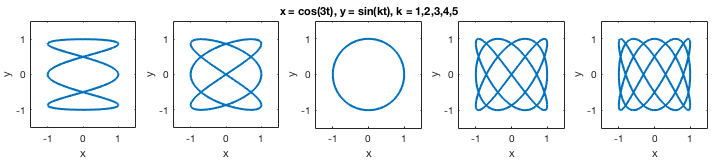
\includegraphics[width=\linewidth]{img/C23p2-18.png}

\begin{lstlisting}
for k = 1:5
    subplot(1,5,k)
    fplot(cos(3*t),sin(k*t),[0,2*pi],'linewidth',2)
    axis equal
    axis([-1.5 1.5 -1.5 1.5])
    xlabel('x'); ylabel('y');
end
subplot(1,5,3)
title('x = cos(3t), y = sin(kt), k = 1,2,3,4,5')
\end{lstlisting}


\begin{lstlisting}
% Computing the integral:
int(sqrt((3*sin(3*t))^2+(5*cos(5*t))^2),t,0,2*pi) % fails
vpa(int(sqrt((3*sin(3*t))^2+(5*cos(5*t))^2),t,0,2*pi)) % returns a numerical approximation
\end{lstlisting}



\vspace{0.2cm}
\hrule
\vspace{0.2cm}

\noindent\textbf{Intersection} \S 17.1
\begin{tcolorbox}
\begin{itemize}
\itemsep0em
    \item Curves $\vec r_1(t), a\leq t\leq b$ and $\vec r_2(t), c\leq t\leq d$ \textbf{intersect} if $\vec r_1(t_0) = \vec r_2(t_1)$ for some $t_0, t_1$ in the domain of the respective paths.
    \item Particles traveling on the paths $\vec r_1(t), a\leq t\leq b$ and $\vec r_2(t), c\leq t\leq d$ \textbf{collide} if $\vec r_1(t_0) = \vec r_2(t_0)$ for some $t_0$ in the domain of both paths.
\end{itemize}
\end{tcolorbox}

\noindent\textbf{Example (intersection)}.
Let $\mb r_1 = (5-3t)\mb i + 2t \mb k$ and $\mb r_2 = (2+6t)\mb i + (2-2t)\mb j$.  Do these lines intersect? 
\vspace{1in}




\vspace{0.2cm}
\hrule
\vspace{0.2cm}

\noindent\textbf{Problem (adding two parameterizations)}.
\begin{questions}

\item
Sometimes motion is a combination of two actions.  Parameterizing the combined motion requires care.
\begin{parts}
\item An ant crawls along the radius from the center of a disk to the outer edge.  The disk has radius $1$ meter and the ant moves at a rate of $1$ centimeter per second.  

Give a parameterization of its radial position, in centimeters.  Include time bounds.

\vfill
\item A disk is rotating counterclockwise about its center at $1$ revolution per second.  Parameterize the path of a point sitting at radius $r$.

\vfill
\item Combine these to find the path of an ant walking steadily outward on a rotating disk.  Assume the ant's motion is completely radial from the perspective of an observer rotating with the disk.

\vfill
\end{parts}

\item

Let $\mb r_1(t) = \cos t\mb i + \sin t\mb j$, a parameterization of the unit circle or a piece of the unit circle.  Let $\mb r_2(t) = t\mb i$, a parameterization of the $x$-axis.  Describe the curve given by $\mb r(t) = \mb r_1(t) + \mb r_2(t)$.
\vfill


\end{questions}



\vspace{0.2cm}
\hrule
\vspace{0.2cm}

\noindent\textbf{Vector fields} \S 17.3

\begin{tcolorbox}
 A function $f: \mathbb{R}^n \rightarrow \mathbb{R}^k$ is a \textbf{vector-valued function} because there are multiple outputs associated with each input.  
    
    The output of the function can be interpreted in two different ways: 
    \begin{itemize} 
    \itemsep0em
    \item as a mapping assigning a vector in $k$-space to each point in $\mathbb{R}^n$.  This is a \textbf{vector field}
    \item as a mapping assigning a point in $k$-space to each point in $\mathbb{R}^n$.  This is a \textbf{parameterization}.
    \end{itemize}
    
To create a representation of a vector field, 
\begin{itemize}
    \itemsep0em
\item we sketch vectors at points in $\mathbb{R}^n$.  
\item Although we only draw the vectors at select points, the
vector field is defined for every point in the domain. \\
\end{itemize}
\end{tcolorbox}



\noindent\textbf{Example (vector field)}.  
\begin{multicols}{2}
Consider
$\mb F(x,y) = x\mb i + 0 \mb j.$  At each point $(x,y)$ in the $xy$-plane we have a corresponding vector $x\mb i$.  We can sketch these vectors.  This is the vector field $\mb F(x,y) = \langle x,0\rangle$.



Sketch this vector field using a unit grid ranging from $-2\leq x \leq 2$, $2\leq y\leq 2$.

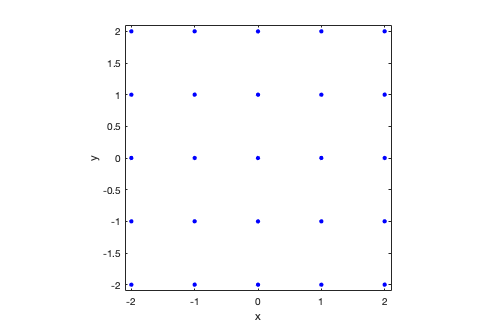
\includegraphics[width=3in]{img/C17grid.png}
\end{multicols}

\noindent\textbf{Question (matching)}.  Match the vector fields \[f(x)\mb i, \quad g(x)\mb j, \quad h(y)\mb i,\quad k(y)\mb j\] to the images below.  %\emph{pollQ}.

\hspace{-0.5in}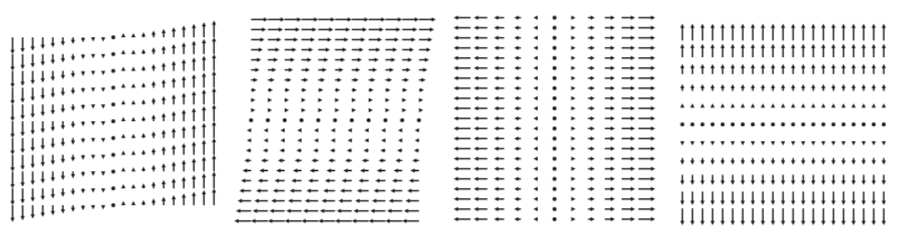
\includegraphics[width=\linewidth]{img/C24p2b-18.png}
\vfill
%

\noindent\textbf{Question (matching)}.  Match the vector fields \[f(x)\mb i+f(x)\mb j,\quad g(x)\mb i - g(x)\mb j,\quad h(y)\mb i + h(y)\mb j,\quad k(y)\mb i - k(y)\mb j\] to the images below. % \emph{pollQ}.

\hspace{-0.5in}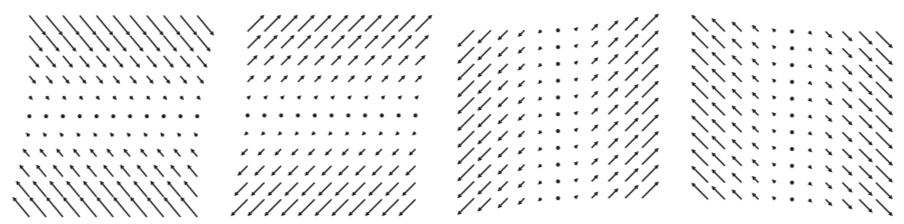
\includegraphics[width=\linewidth]{img/C24p3b-18.png}

\vfill



\noindent\textbf{Examples (vector fields to know)}. 

$\mb F_i = \mb r$, $\mb F_{ii} = \frac{\mb r}{\Vert \mb r\Vert}$.  $\mb F_{iii} = x\mb j$.  $\mb F_{iv} = y\mb i - x\mb j.$


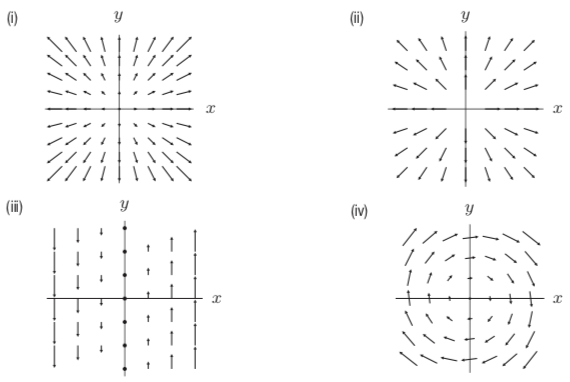
\includegraphics[width=0.8\linewidth]{img/C24p4-18.png}

\vfill




\vspace{0.2cm}
\hrule
\vspace{0.2cm}

\begin{tcolorbox}


\noindent\textbf{Force fields} are a common type of vector field.  Because forces have a direction as well as a magnitude, and force fields act at each point in space, a vector field is an appropriate representation. 
\end{tcolorbox}

Below is a visualization of a magnetic field.  The vectors themselves are not quite visible.  Each iron filing is aligned with the magnetic field.  However the length of filings does not vary with the strength of the field, as it would it we were drawing in vectors:

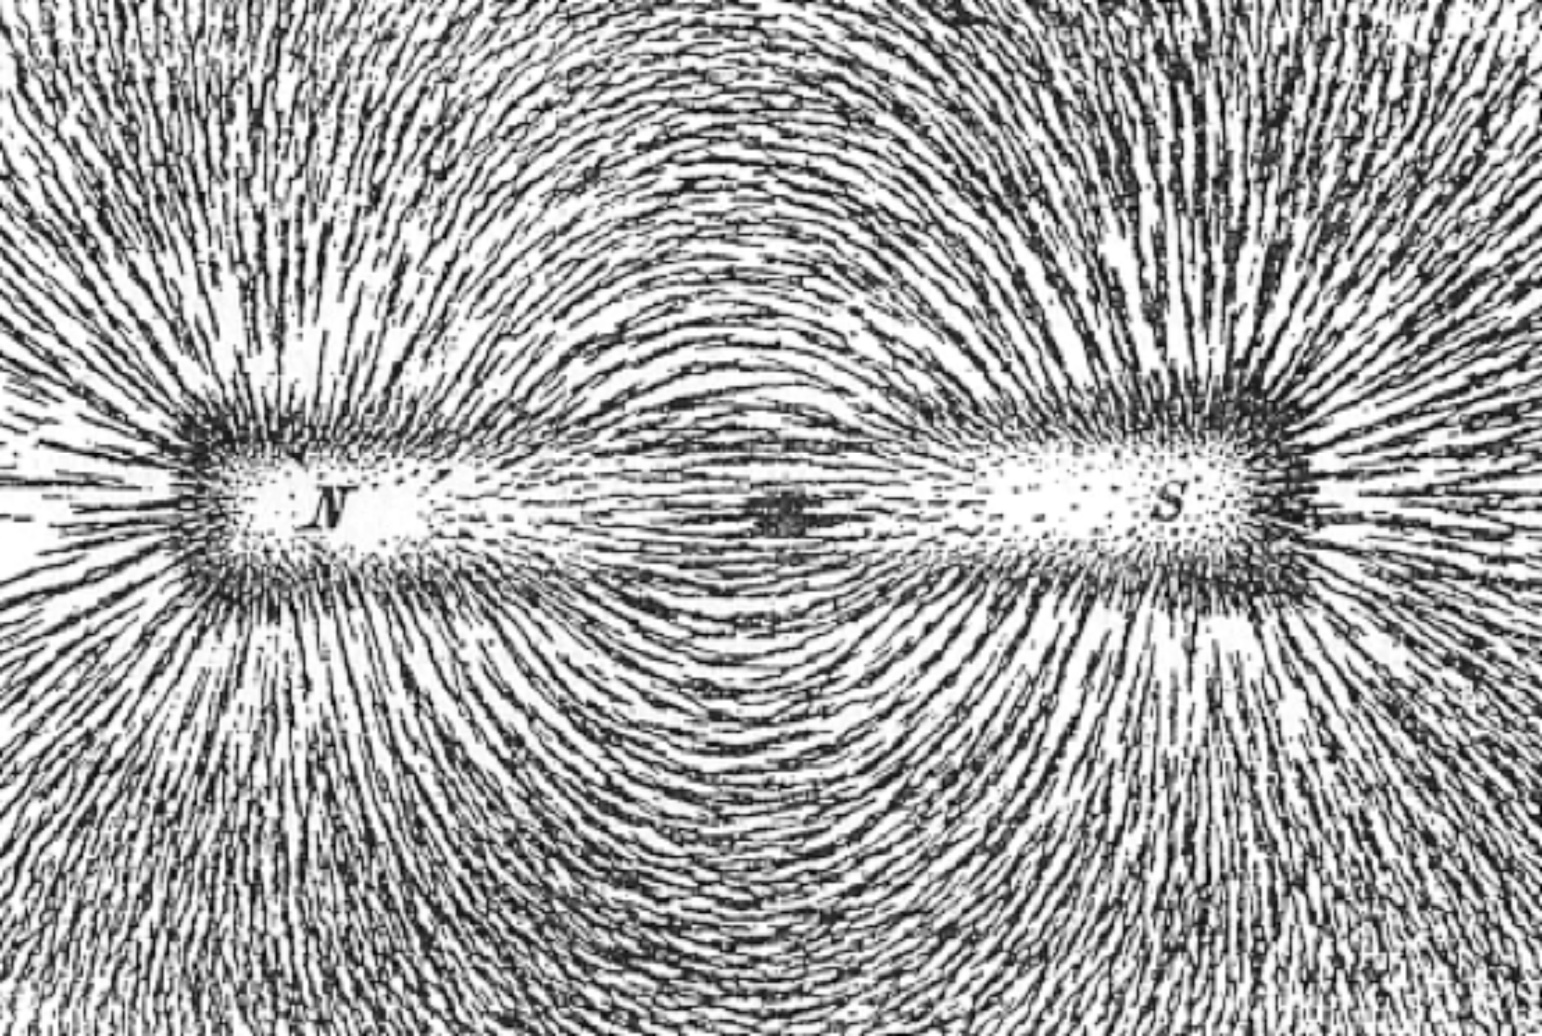
\includegraphics[width=3in]{img/C24p5.png}

\url{http://www.txessrevolution.org/MagneticSun_Info}

\vspace{0.1cm}

\noindent\textbf{Example: gravitational force}

$\displaystyle\mb F(\mb r) = -\frac{GMm\mb r}{\Vert \mb r\Vert^3}$.  $\mb r = \langle x, y, z\rangle$, so this is a compact notation for
$\displaystyle\mb F(\mb r) = -GMm(\frac{x}{(x^2+y^2+z^2)^{3/2}}\mb i+\frac{y}{(x^2+y^2+z^2)^{3/2}}\mb j + \frac{z}{(x^2+y^2+z^2)^{3/2}}\mb k$
 
$\mb F(\mb r)$ is a radial vector field where all vectors point towards the origin.
 
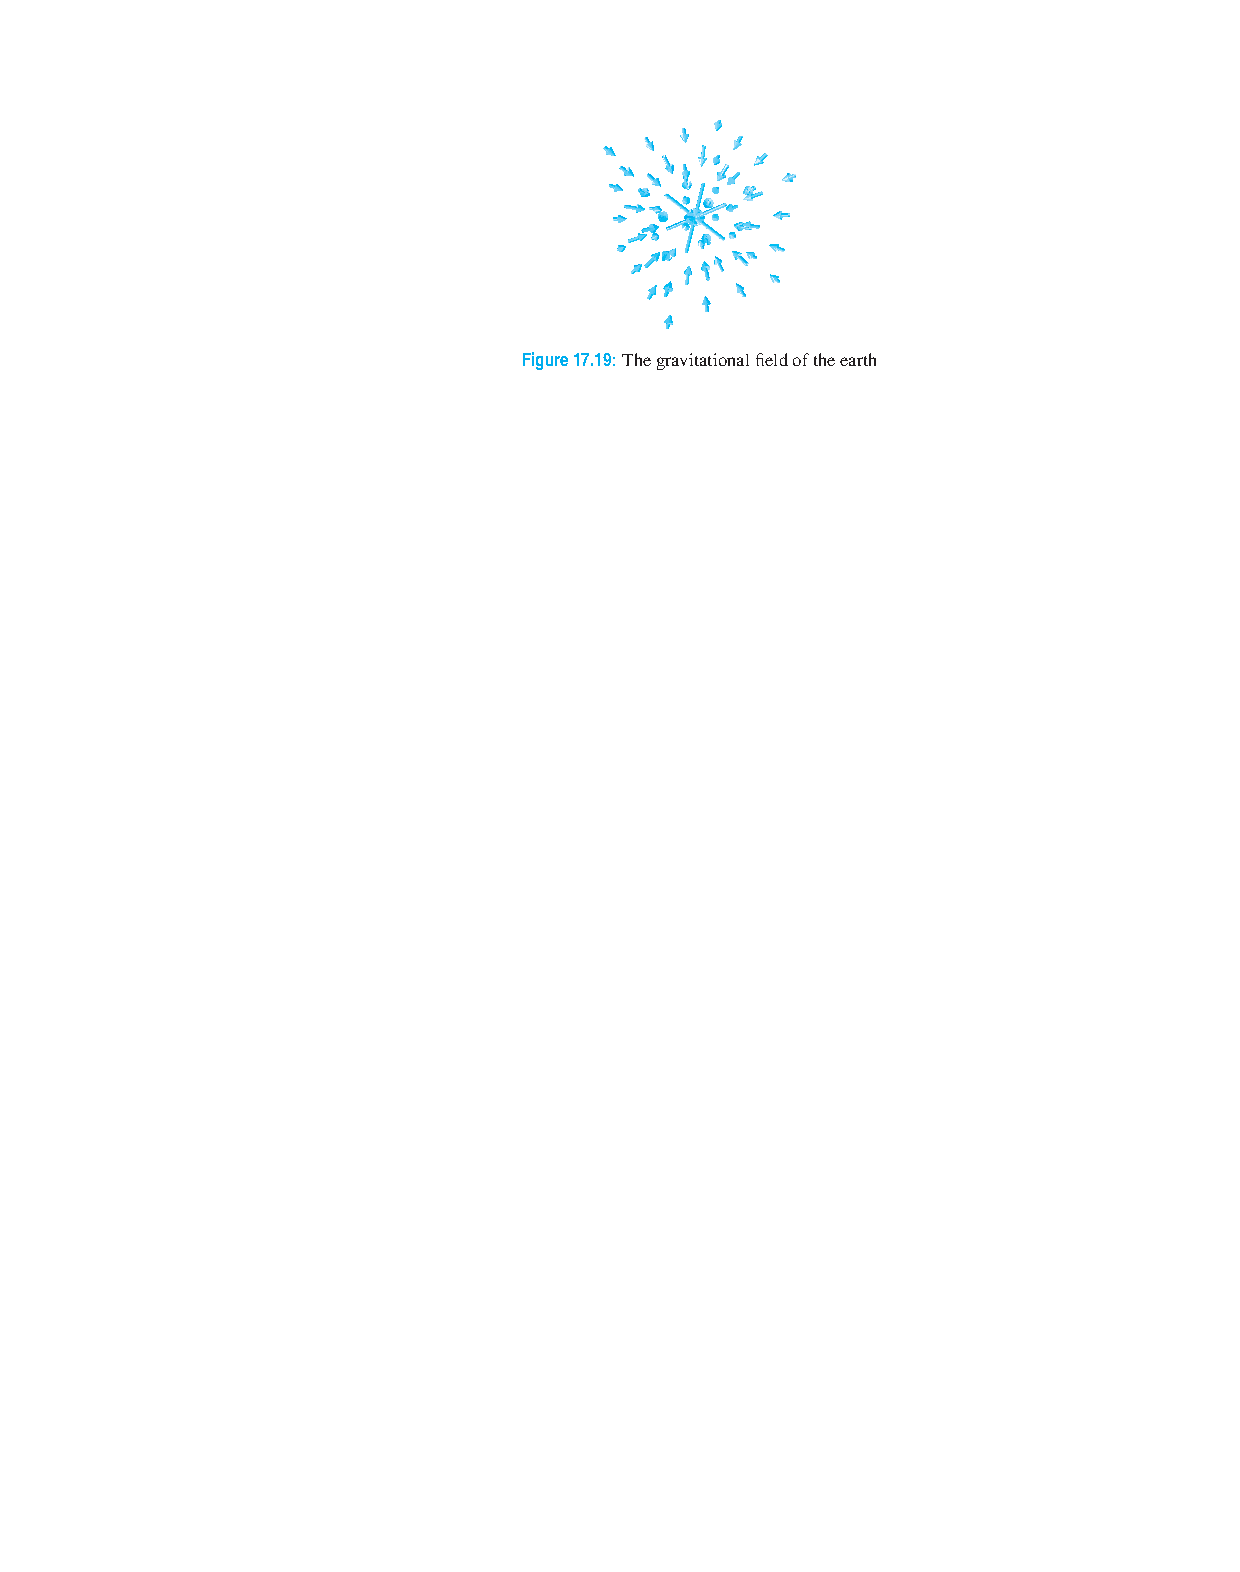
\includegraphics{img/N24_p4.pdf}

\vspace{0.1cm}

\noindent\textbf{Example (dolphin motion)}.
Velocity vectors of the water motion as a dolphin swims are shown (with their length indicated by color) at nine different timepoints.

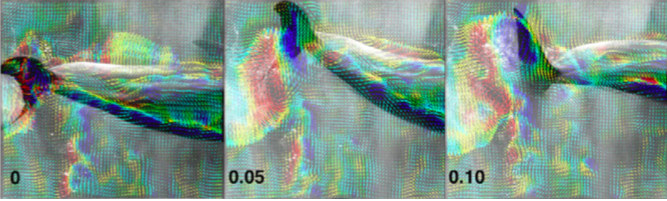
\includegraphics[width=0.8\linewidth]{img/C24p1b-18.png}

\cite{fish2014measurement}
\vfill




\noindent\textbf{Example (wind velocity)}.

Here is an example where vectors are indicating the wind velocity near Hurricane Katrina (measured by a satellite in Aug 2005):

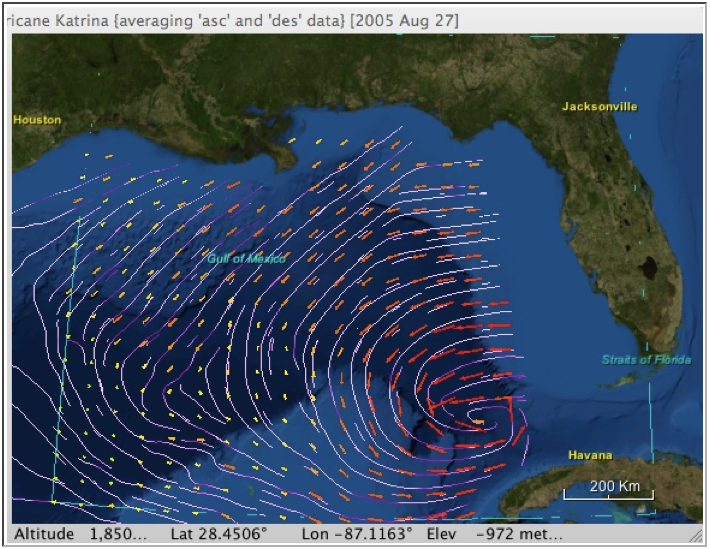
\includegraphics[width=5in]{img/N24_p2.png}

\url{https://people.eecs.ku.edu/~miller/WorldWindProjects/VectorFieldVis/5DayKatrinaNoGrid.html}



The length of each vector indicates its relative magnitude.  The vectors are color coded by magnitude: red is high speed, and yellow low.  


\vspace{0.2cm}
\hrule
\vspace{0.2cm}




\bibliographystyle{plainnat}
\bibliography{main}










\end{document}